%%%%%%%%%%%%%%%%%%%%%%%%%%%%%%%%%%%%%%%%%
% The Legrand Orange Book
% LaTeX Template
% Version 2.0 (9/2/15)
%
% This template has been downloaded from:
% http://www.LaTeXTemplates.com
%
% Mathias Legrand (legrand.mathias@gmail.com) with modifications by:
% Vel (vel@latextemplates.com)
%
% License:
% CC BY-NC-SA 3.0 (http://creativecommons.org/licenses/by-nc-sa/3.0/)
%
% Compiling this template:
% This template uses biber for its bibliography and makeindex for its index.
% When you first open the template, compile it from the command line with the 
% commands below to make sure your LaTeX distribution is configured correctly:
%
% 1) pdflatex main
% 2) makeindex main.idx -s StyleInd.ist
% 3) biber main
% 4) pdflatex main x 2
%
% After this, when you wish to update the bibliography/index use the appropriate
% command above and make sure to compile with pdflatex several times 
% afterwards to propagate your changes to the document.
%
% This template also uses a number of packages which may need to be
% updated to the newest versions for the template to compile. It is strongly
% recommended you update your LaTeX distribution if you have any
% compilation errors.
%
% Important note:
% Chapter heading images should have a 2:1 width:height ratio,
% e.g. 920px width and 460px height.
%
%%%%%%%%%%%%%%%%%%%%%%%%%%%%%%%%%%%%%%%%%

%----------------------------------------------------------------------------------------
%	PACKAGES AND OTHER DOCUMENT CONFIGURATIONS
%----------------------------------------------------------------------------------------

\documentclass[11pt,fleqn]{book} % Default font size and left-justified equations

%----------------------------------------------------------------------------------------

%%%%%%%%%%%%%%%%%%%%%%%%%%%%%%%%%%%%%%%%%
% The Legrand Orange Book
% Structural Definitions File
% Version 2.0 (9/2/15)
%
% Original author:
% Mathias Legrand (legrand.mathias@gmail.com) with modifications by:
% Vel (vel@latextemplates.com)
% 
% This file has been downloaded from:
% http://www.LaTeXTemplates.com
%
% License:
% CC BY-NC-SA 3.0 (http://creativecommons.org/licenses/by-nc-sa/3.0/)
%
%%%%%%%%%%%%%%%%%%%%%%%%%%%%%%%%%%%%%%%%%

%----------------------------------------------------------------------------------------
%	VARIOUS REQUIRED PACKAGES AND CONFIGURATIONS
%----------------------------------------------------------------------------------------

\usepackage[top=3cm,bottom=3cm,left=3cm,right=3cm,headsep=10pt,a4paper]{geometry} % Page margins

\usepackage{graphicx} % Required for including pictures
\graphicspath{{Pictures/}} % Specifies the directory where pictures are stored

\usepackage{float}
\usepackage{svg}

\usepackage{lipsum} % Inserts dummy text

\usepackage{tikz} % Required for drawing custom shapes

\usepackage[english]{babel} % English language/hyphenation

\usepackage{enumitem} % Customize lists
\setlist{nolistsep} % Reduce spacing between bullet points and numbered lists

\usepackage{booktabs} % Required for nicer horizontal rules in tables

\usepackage{xcolor} % Required for specifying colors by name
\definecolor{ocre}{RGB}{243,102,25} % Define the orange color used for highlighting throughout the book


%----------------------------------------------------------------------------------------
%	FONTS
%----------------------------------------------------------------------------------------

\usepackage{avant} % Use the Avantgarde font for headings
%\usepackage{times} % Use the Times font for headings
\usepackage{mathptmx} % Use the Adobe Times Roman as the default text font together with math symbols from the Sym­bol, Chancery and Com­puter Modern fonts

\usepackage{microtype} % Slightly tweak font spacing for aesthetics
\usepackage[utf8]{inputenc} % Required for including letters with accents
\usepackage[T1]{fontenc} % Use 8-bit encoding that has 256 glyphs

\usepackage{mathtools}
\usepackage{soul}
%----------------------------------------------------------------------------------------
%	BIBLIOGRAPHY AND INDEX
%----------------------------------------------------------------------------------------

\usepackage[style=alphabetic,citestyle=numeric,sorting=nyt,sortcites=true,autopunct=true,babel=hyphen,hyperref=true,abbreviate=false,backref=true,backend=biber]{biblatex}
\addbibresource{bibliography.bib} % BibTeX bibliography file
\defbibheading{bibempty}{}

\usepackage{calc} % For simpler calculation - used for spacing the index letter headings correctly
\usepackage{makeidx} % Required to make an index
\makeindex % Tells LaTeX to create the files required for indexing

%----------------------------------------------------------------------------------------
%	MAIN TABLE OF CONTENTS
%----------------------------------------------------------------------------------------

\usepackage{titletoc} % Required for manipulating the table of contents

\contentsmargin{0cm} % Removes the default margin

% Part text styling
\titlecontents{part}[0cm]
{\addvspace{20pt}\centering\large\bfseries}
{}
{}
{}

% Chapter text styling
\titlecontents{chapter}[1.25cm] % Indentation
{\addvspace{12pt}\large\sffamily\bfseries} % Spacing and font options for chapters
{\color{ocre!60}\contentslabel[\Large\thecontentslabel]{1.25cm}\color{ocre}} % Chapter number
{\color{ocre}}  
{\color{ocre!60}\normalsize\;\titlerule*[.5pc]{.}\;\thecontentspage} % Page number

% Section text styling
\titlecontents{section}[1.25cm] % Indentation
{\addvspace{3pt}\sffamily\bfseries} % Spacing and font options for sections
{\contentslabel[\thecontentslabel]{1.25cm}} % Section number
{}
{\hfill\color{black}\thecontentspage} % Page number
[]

% Subsection text styling
\titlecontents{subsection}[1.25cm] % Indentation
{\addvspace{1pt}\sffamily\small} % Spacing and font options for subsections
{\contentslabel[\thecontentslabel]{1.25cm}} % Subsection number
{}
{\ \titlerule*[.5pc]{.}\;\thecontentspage} % Page number
[]

% List of figures
\titlecontents{figure}[0em]
{\addvspace{-5pt}\sffamily}
{\thecontentslabel\hspace*{1em}}
{}
{\ \titlerule*[.5pc]{.}\;\thecontentspage}
[]

% List of tables
\titlecontents{table}[0em]
{\addvspace{-5pt}\sffamily}
{\thecontentslabel\hspace*{1em}}
{}
{\ \titlerule*[.5pc]{.}\;\thecontentspage}
[]

%----------------------------------------------------------------------------------------
%	MINI TABLE OF CONTENTS IN PART HEADS
%----------------------------------------------------------------------------------------

% Chapter text styling
\titlecontents{lchapter}[0em] % Indenting
{\addvspace{15pt}\large\sffamily\bfseries} % Spacing and font options for chapters
{\color{ocre}\contentslabel[\Large\thecontentslabel]{1.25cm}\color{ocre}} % Chapter number
{}  
{\color{ocre}\normalsize\sffamily\bfseries\;\titlerule*[.5pc]{.}\;\thecontentspage} % Page number

% Section text styling
\titlecontents{lsection}[0em] % Indenting
{\sffamily\small} % Spacing and font options for sections
{\contentslabel[\thecontentslabel]{1.25cm}} % Section number
{}
{}

% Subsection text styling
\titlecontents{lsubsection}[.5em] % Indentation
{\normalfont\footnotesize\sffamily} % Font settings
{}
{}
{}

%----------------------------------------------------------------------------------------
%	PAGE HEADERS
%----------------------------------------------------------------------------------------

\usepackage{fancyhdr} % Required for header and footer configuration

\pagestyle{fancy}
\renewcommand{\chaptermark}[1]{\markboth{\sffamily\normalsize\bfseries\chaptername\ \thechapter.\ #1}{}} % Chapter text font settings
\renewcommand{\sectionmark}[1]{\markright{\sffamily\normalsize\thesection\hspace{5pt}#1}{}} % Section text font settings
\fancyhf{} \fancyhead[LE,RO]{\sffamily\normalsize\thepage} % Font setting for the page number in the header
\fancyhead[LO]{\rightmark} % Print the nearest section name on the left side of odd pages
\fancyhead[RE]{\leftmark} % Print the current chapter name on the right side of even pages
\renewcommand{\headrulewidth}{0.5pt} % Width of the rule under the header
\addtolength{\headheight}{2.5pt} % Increase the spacing around the header slightly
\renewcommand{\footrulewidth}{0pt} % Removes the rule in the footer
\fancypagestyle{plain}{\fancyhead{}\renewcommand{\headrulewidth}{0pt}} % Style for when a plain pagestyle is specified

% Removes the header from odd empty pages at the end of chapters
\makeatletter
\renewcommand{\cleardoublepage}{
\clearpage\ifodd\c@page\else
\hbox{}
\vspace*{\fill}
\thispagestyle{empty}
\newpage
\fi}

%----------------------------------------------------------------------------------------
%	THEOREM STYLES
%----------------------------------------------------------------------------------------

\usepackage{amsmath,amsfonts,amssymb,amsthm} % For math equations, theorems, symbols, etc

\newcommand{\intoo}[2]{\mathopen{]}#1\,;#2\mathclose{[}}
\newcommand{\ud}{\mathop{\mathrm{{}d}}\mathopen{}}
\newcommand{\intff}[2]{\mathopen{[}#1\,;#2\mathclose{]}}
\newtheorem{notation}{Notation}[chapter]

% Boxed/framed environments
\newtheoremstyle{ocrenumbox}% % Theorem style name
{0pt}% Space above
{0pt}% Space below
{\normalfont}% % Body font
{}% Indent amount
{\small\bf\sffamily\color{ocre}}% % Theorem head font
{\;}% Punctuation after theorem head
{0.25em}% Space after theorem head
{\small\sffamily\color{ocre}\thmname{#1}\nobreakspace\thmnumber{\@ifnotempty{#1}{}\@upn{#2}}% Theorem text (e.g. Theorem 2.1)
\thmnote{\nobreakspace\the\thm@notefont\sffamily\bfseries\color{black}---\nobreakspace#3.}} % Optional theorem note
\renewcommand{\qedsymbol}{$\blacksquare$}% Optional qed square

\newtheoremstyle{blacknumex}% Theorem style name
{5pt}% Space above
{5pt}% Space below
{\normalfont}% Body font
{} % Indent amount
{\small\bf\sffamily}% Theorem head font
{\;}% Punctuation after theorem head
{0.25em}% Space after theorem head
{\small\sffamily{\tiny\ensuremath{\blacksquare}}\nobreakspace\thmname{#1}\nobreakspace\thmnumber{\@ifnotempty{#1}{}\@upn{#2}}% Theorem text (e.g. Theorem 2.1)
\thmnote{\nobreakspace\the\thm@notefont\sffamily\bfseries---\nobreakspace#3.}}% Optional theorem note

\newtheoremstyle{blacknumbox} % Theorem style name
{0pt}% Space above
{0pt}% Space below
{\normalfont}% Body font
{}% Indent amount
{\small\bf\sffamily}% Theorem head font
{\;}% Punctuation after theorem head
{0.25em}% Space after theorem head
{\small\sffamily\thmname{#1}\nobreakspace\thmnumber{\@ifnotempty{#1}{}\@upn{#2}}% Theorem text (e.g. Theorem 2.1)
\thmnote{\nobreakspace\the\thm@notefont\sffamily\bfseries---\nobreakspace#3.}}% Optional theorem note

% Non-boxed/non-framed environments
\newtheoremstyle{ocrenum}% % Theorem style name
{5pt}% Space above
{5pt}% Space below
{\normalfont}% % Body font
{}% Indent amount
{\small\bf\sffamily\color{ocre}}% % Theorem head font
{\;}% Punctuation after theorem head
{0.25em}% Space after theorem head
{\small\sffamily\color{ocre}\thmname{#1}\nobreakspace\thmnumber{\@ifnotempty{#1}{}\@upn{#2}}% Theorem text (e.g. Theorem 2.1)
\thmnote{\nobreakspace\the\thm@notefont\sffamily\bfseries\color{black}---\nobreakspace#3.}} % Optional theorem note
\renewcommand{\qedsymbol}{$\blacksquare$}% Optional qed square
\makeatother

% Defines the theorem text style for each type of theorem to one of the three styles above
\newcounter{dummy} 
\numberwithin{dummy}{section}
\theoremstyle{ocrenumbox}
\newtheorem{theoremeT}[dummy]{Theorem}
\newtheorem{problem}{Problem}[chapter]
\newtheorem{exerciseT}{Exercise}[chapter]
\theoremstyle{blacknumex}
\newtheorem{exampleT}{Example}[chapter]
\theoremstyle{blacknumbox}
\newtheorem{vocabulary}{Vocabulary}[chapter]
\newtheorem{definitionT}{Definition}[section]
\newtheorem{corollaryT}[dummy]{Corollary}
\theoremstyle{ocrenum}
\newtheorem{proposition}[dummy]{Proposition}

%----------------------------------------------------------------------------------------
%	DEFINITION OF COLORED BOXES
%----------------------------------------------------------------------------------------

\RequirePackage[framemethod=default]{mdframed} % Required for creating the theorem, definition, exercise and corollary boxes

% Theorem box
\newmdenv[skipabove=7pt,
skipbelow=7pt,
backgroundcolor=black!5,
linecolor=ocre,
innerleftmargin=5pt,
innerrightmargin=5pt,
innertopmargin=5pt,
leftmargin=0cm,
rightmargin=0cm,
innerbottommargin=5pt]{tBox}

% Exercise box	  
\newmdenv[skipabove=7pt,
skipbelow=7pt,
rightline=false,
leftline=true,
topline=false,
bottomline=false,
backgroundcolor=ocre!10,
linecolor=ocre,
innerleftmargin=5pt,
innerrightmargin=5pt,
innertopmargin=5pt,
innerbottommargin=5pt,
leftmargin=0cm,
rightmargin=0cm,
linewidth=4pt]{eBox}	

% Definition box
\newmdenv[skipabove=7pt,
skipbelow=7pt,
rightline=false,
leftline=true,
topline=false,
bottomline=false,
linecolor=ocre,
innerleftmargin=5pt,
innerrightmargin=5pt,
innertopmargin=0pt,
leftmargin=0cm,
rightmargin=0cm,
linewidth=4pt,
innerbottommargin=0pt]{dBox}	

% Corollary box
\newmdenv[skipabove=7pt,
skipbelow=7pt,
rightline=false,
leftline=true,
topline=false,
bottomline=false,
linecolor=gray,
backgroundcolor=black!5,
innerleftmargin=5pt,
innerrightmargin=5pt,
innertopmargin=5pt,
leftmargin=0cm,
rightmargin=0cm,
linewidth=4pt,
innerbottommargin=5pt]{cBox}

% Creates an environment for each type of theorem and assigns it a theorem text style from the "Theorem Styles" section above and a colored box from above
\newenvironment{theorem}{\begin{tBox}\begin{theoremeT}}{\end{theoremeT}\end{tBox}}
\newenvironment{exercise}{\begin{eBox}\begin{exerciseT}}{\hfill{\color{ocre}\tiny\ensuremath{\blacksquare}}\end{exerciseT}\end{eBox}}				  
\newenvironment{definition}{\begin{dBox}\begin{definitionT}}{\end{definitionT}\end{dBox}}	
\newenvironment{example}{\begin{exampleT}}{\hfill{\tiny\ensuremath{\blacksquare}}\end{exampleT}}		
\newenvironment{corollary}{\begin{cBox}\begin{corollaryT}}{\end{corollaryT}\end{cBox}}	

%----------------------------------------------------------------------------------------
%	REMARK ENVIRONMENT
%----------------------------------------------------------------------------------------

\newenvironment{remark}{\par\vspace{10pt}\small % Vertical white space above the remark and smaller font size
\begin{list}{}{
\leftmargin=35pt % Indentation on the left
\rightmargin=25pt}\item\ignorespaces % Indentation on the right
\makebox[-2.5pt]{\begin{tikzpicture}[overlay]
\node[draw=ocre!60,line width=1pt,circle,fill=ocre!25,font=\sffamily\bfseries,inner sep=2pt,outer sep=0pt] at (-15pt,0pt){\textcolor{ocre}{R}};\end{tikzpicture}} % Orange R in a circle
\advance\baselineskip -1pt}{\end{list}\vskip5pt} % Tighter line spacing and white space after remark

%----------------------------------------------------------------------------------------
%	SECTION NUMBERING IN THE MARGIN
%----------------------------------------------------------------------------------------

\makeatletter
\renewcommand{\@seccntformat}[1]{\llap{\textcolor{ocre}{\csname the#1\endcsname}\hspace{1em}}}                    
\renewcommand{\section}{\@startsection{section}{1}{\z@}
{-4ex \@plus -1ex \@minus -.4ex}
{1ex \@plus.2ex }
{\normalfont\large\sffamily\bfseries}}
\renewcommand{\subsection}{\@startsection {subsection}{2}{\z@}
{-3ex \@plus -0.1ex \@minus -.4ex}
{0.5ex \@plus.2ex }
{\normalfont\sffamily\bfseries}}
\renewcommand{\subsubsection}{\@startsection {subsubsection}{3}{\z@}
{-2ex \@plus -0.1ex \@minus -.2ex}
{.2ex \@plus.2ex }
{\normalfont\small\sffamily\bfseries}}                        
\renewcommand\paragraph{\@startsection{paragraph}{4}{\z@}
{-2ex \@plus-.2ex \@minus .2ex}
{.1ex}
{\normalfont\small\sffamily\bfseries}}

%----------------------------------------------------------------------------------------
%	PART HEADINGS
%----------------------------------------------------------------------------------------

% numbered part in the table of contents
\newcommand{\@mypartnumtocformat}[2]{%
\setlength\fboxsep{0pt}%
\noindent\colorbox{ocre!20}{\strut\parbox[c][.7cm]{\ecart}{\color{ocre!70}\Large\sffamily\bfseries\centering#1}}\hskip\esp\colorbox{ocre!40}{\strut\parbox[c][.7cm]{\linewidth-\ecart-\esp}{\Large\sffamily\centering#2}}}%
%%%%%%%%%%%%%%%%%%%%%%%%%%%%%%%%%%
% unnumbered part in the table of contents
\newcommand{\@myparttocformat}[1]{%
\setlength\fboxsep{0pt}%
\noindent\colorbox{ocre!40}{\strut\parbox[c][.7cm]{\linewidth}{\Large\sffamily\centering#1}}}%
%%%%%%%%%%%%%%%%%%%%%%%%%%%%%%%%%%
\newlength\esp
\setlength\esp{4pt}
\newlength\ecart
\setlength\ecart{1.2cm-\esp}
\newcommand{\thepartimage}{}%
\newcommand{\partimage}[1]{\renewcommand{\thepartimage}{#1}}%
\def\@part[#1]#2{%
\ifnum \c@secnumdepth >-2\relax%
\refstepcounter{part}%
\addcontentsline{toc}{part}{\texorpdfstring{\protect\@mypartnumtocformat{\thepart}{#1}}{\partname~\thepart\ ---\ #1}}
\else%
\addcontentsline{toc}{part}{\texorpdfstring{\protect\@myparttocformat{#1}}{#1}}%
\fi%
\startcontents%
\markboth{}{}%
{\thispagestyle{empty}%
\begin{tikzpicture}[remember picture,overlay]%
\node at (current page.north west){\begin{tikzpicture}[remember picture,overlay]%	
\fill[ocre!20](0cm,0cm) rectangle (\paperwidth,-\paperheight);
\node[anchor=north] at (4cm,-3.25cm){\color{ocre!40}\fontsize{220}{100}\sffamily\bfseries\@Roman\c@part}; 
\node[anchor=south east] at (\paperwidth-1cm,-\paperheight+1cm){\parbox[t][][t]{8.5cm}{
\printcontents{l}{0}{\setcounter{tocdepth}{1}}%
}};
\node[anchor=north east] at (\paperwidth-1.5cm,-3.25cm){\parbox[t][][t]{15cm}{\strut\raggedleft\color{white}\fontsize{30}{30}\sffamily\bfseries#2}};
\end{tikzpicture}};
\end{tikzpicture}}%
\@endpart}
\def\@spart#1{%
\startcontents%
\phantomsection
{\thispagestyle{empty}%
\begin{tikzpicture}[remember picture,overlay]%
\node at (current page.north west){\begin{tikzpicture}[remember picture,overlay]%	
\fill[ocre!20](0cm,0cm) rectangle (\paperwidth,-\paperheight);
\node[anchor=north east] at (\paperwidth-1.5cm,-3.25cm){\parbox[t][][t]{15cm}{\strut\raggedleft\color{white}\fontsize{30}{30}\sffamily\bfseries#1}};
\end{tikzpicture}};
\end{tikzpicture}}
\addcontentsline{toc}{part}{\texorpdfstring{%
\setlength\fboxsep{0pt}%
\noindent\protect\colorbox{ocre!40}{\strut\protect\parbox[c][.7cm]{\linewidth}{\Large\sffamily\protect\centering #1\quad\mbox{}}}}{#1}}%
\@endpart}
\def\@endpart{\vfil\newpage
\if@twoside
\if@openright
\null
\thispagestyle{empty}%
\newpage
\fi
\fi
\if@tempswa
\twocolumn
\fi}

%----------------------------------------------------------------------------------------
%	CHAPTER HEADINGS
%----------------------------------------------------------------------------------------

\newcommand{\thechapterimage}{}%
\newcommand{\chapterimage}[1]{\renewcommand{\thechapterimage}{#1}}%
\def\@makechapterhead#1{%
{\parindent \z@ \raggedright \normalfont
\ifnum \c@secnumdepth >\m@ne
\if@mainmatter
\begin{tikzpicture}[remember picture,overlay]
\node at (current page.north west)
{\begin{tikzpicture}[remember picture,overlay]
\node[anchor=north west,inner sep=0pt] at (0,0) {\includegraphics[width=\paperwidth]{\thechapterimage}};
\draw[anchor=west] (\Gm@lmargin,-9cm) node [line width=2pt,rounded corners=15pt,draw=ocre,fill=white,fill opacity=0.5,inner sep=15pt]{\strut\makebox[22cm]{}};
\draw[anchor=west] (\Gm@lmargin+.3cm,-9cm) node {\huge\sffamily\bfseries\color{black}\thechapter. #1\strut};
\end{tikzpicture}};
\end{tikzpicture}
\else
\begin{tikzpicture}[remember picture,overlay]
\node at (current page.north west)
{\begin{tikzpicture}[remember picture,overlay]
\node[anchor=north west,inner sep=0pt] at (0,0) {\includegraphics[width=\paperwidth]{\thechapterimage}};
\draw[anchor=west] (\Gm@lmargin,-9cm) node [line width=2pt,rounded corners=15pt,draw=ocre,fill=white,fill opacity=0.5,inner sep=15pt]{\strut\makebox[22cm]{}};
\draw[anchor=west] (\Gm@lmargin+.3cm,-9cm) node {\huge\sffamily\bfseries\color{black}#1\strut};
\end{tikzpicture}};
\end{tikzpicture}
\fi\fi\par\vspace*{270\p@}}}

%-------------------------------------------

\def\@makeschapterhead#1{%
\begin{tikzpicture}[remember picture,overlay]
\node at (current page.north west)
{\begin{tikzpicture}[remember picture,overlay]
\node[anchor=north west,inner sep=0pt] at (0,0) {\includegraphics[width=\paperwidth]{\thechapterimage}};
\draw[anchor=west] (\Gm@lmargin,-9cm) node [line width=2pt,rounded corners=15pt,draw=ocre,fill=white,fill opacity=0.5,inner sep=15pt]{\strut\makebox[22cm]{}};
\draw[anchor=west] (\Gm@lmargin+.3cm,-9cm) node {\huge\sffamily\bfseries\color{black}#1\strut};
\end{tikzpicture}};
\end{tikzpicture}
\par\vspace*{270\p@}}
\makeatother

%----------------------------------------------------------------------------------------
%	HYPERLINKS IN THE DOCUMENTS
%----------------------------------------------------------------------------------------

\usepackage{hyperref}
\hypersetup{hidelinks,backref=true,pagebackref=true,hyperindex=true,colorlinks=false,breaklinks=true,urlcolor= ocre,bookmarks=true,bookmarksopen=false,pdftitle={Title},pdfauthor={Author}}
\usepackage{bookmark}
\bookmarksetup{
open,
numbered,
addtohook={%
\ifnum\bookmarkget{level}=0 % chapter
\bookmarksetup{bold}%
\fi
\ifnum\bookmarkget{level}=-1 % part
\bookmarksetup{color=ocre,bold}%
\fi
}
}

\newcommand\ol[1]{{\setul{-0.9em}{}\ul{#1}}} % Insert the commands.tex file which contains the majority of the structure behind the template

\begin{document}

%----------------------------------------------------------------------------------------
%	TITLE PAGE
%----------------------------------------------------------------------------------------

\begingroup
\thispagestyle{empty}
\begin{tikzpicture}[remember picture,overlay]
\coordinate [below=12cm] (midpoint) at (current page.north);
\node at (current page.north west)
{\begin{tikzpicture}[remember picture,overlay]
\node[anchor=north west,inner sep=0pt] at (0,0) {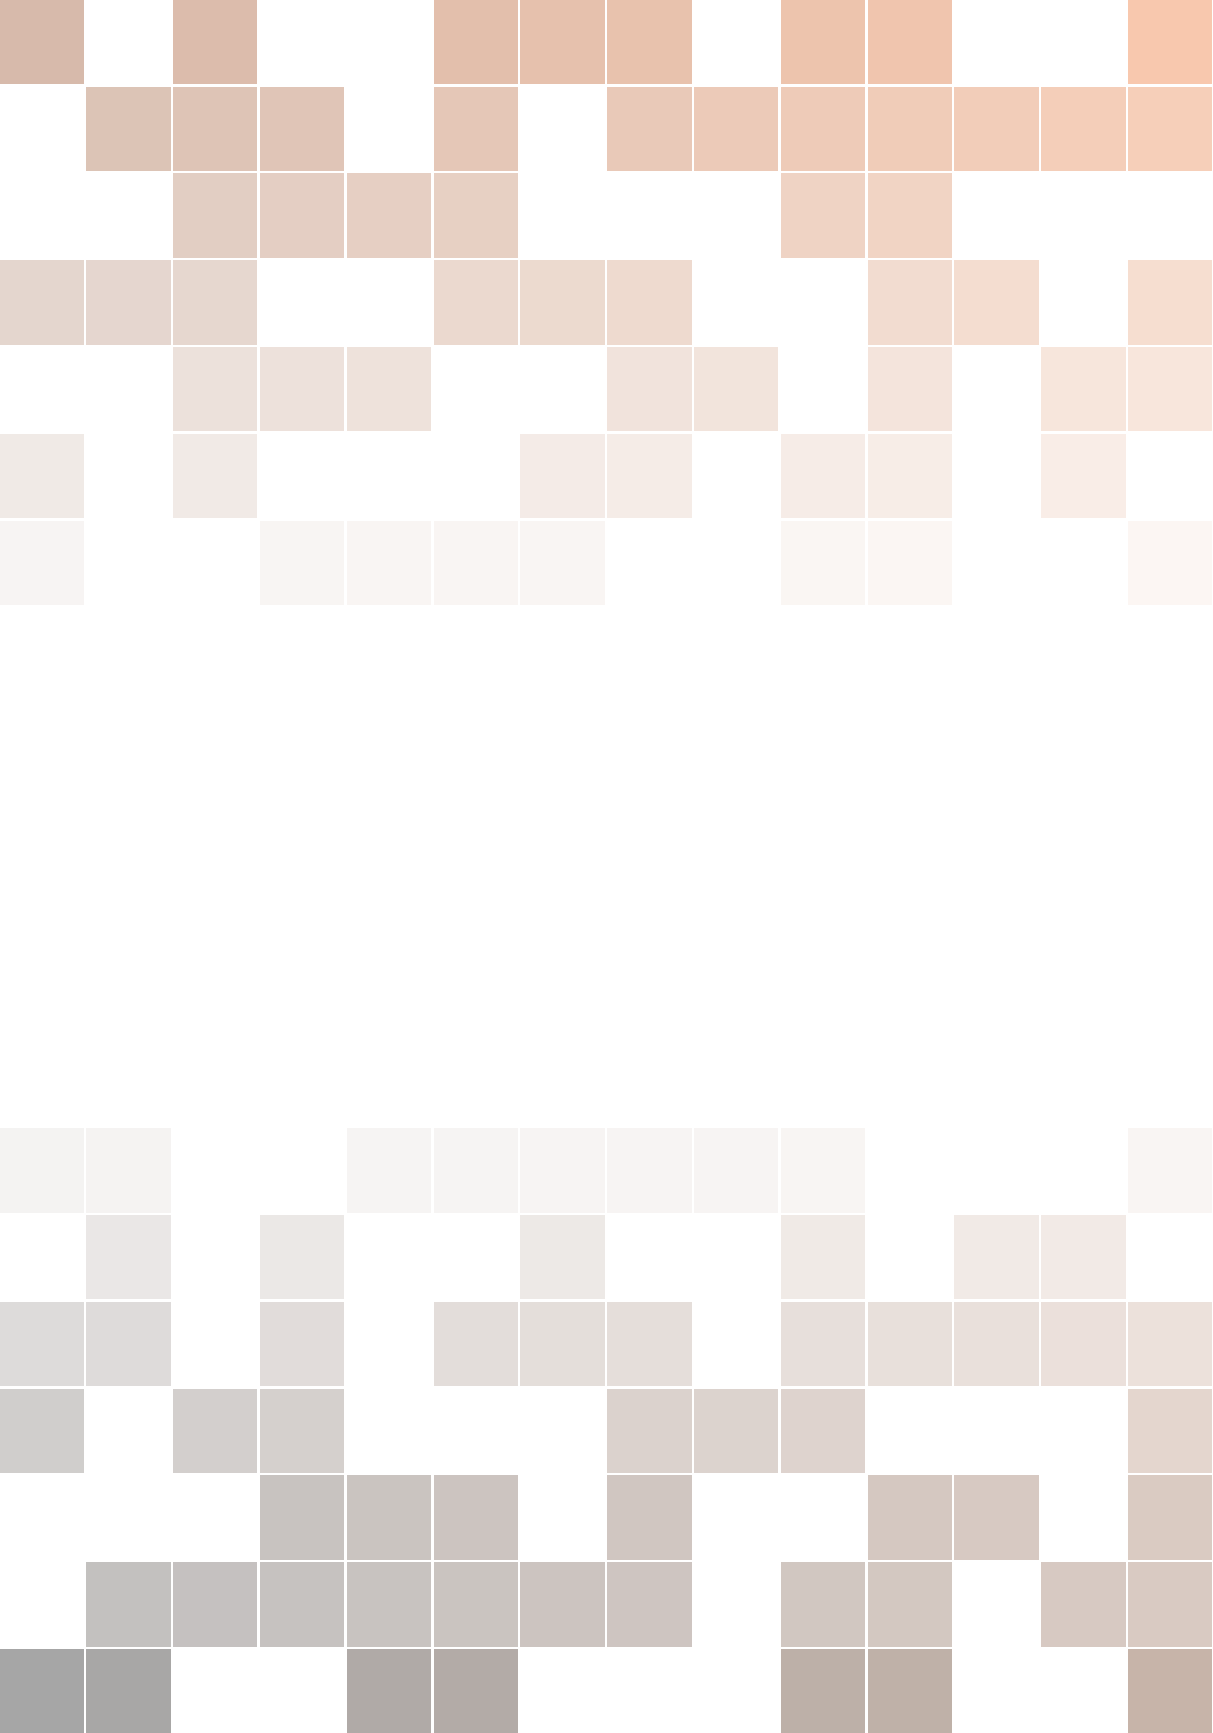
\includegraphics[width=\paperwidth]{template/background}}; % Background image
\draw[anchor=north] (midpoint) node [fill=ocre!30!white,fill opacity=0.6,text opacity=1,inner sep=1cm]{\Huge\centering\bfseries\sffamily\parbox[c][][t]{\paperwidth}{\centering Genética Quantitativa\\[15pt] % Book title
{\Large Aulas e Anotações}\\[20pt] % Subtitle
{\huge D.A.S}}}; % Author name
\end{tikzpicture}};
\end{tikzpicture}
\vfill
\endgroup

%----------------------------------------------------------------------------------------
%	COPYRIGHT PAGE
%----------------------------------------------------------------------------------------

\newpage
~\vfill
\thispagestyle{empty}

\noindent Copyleft - 2018 D.A.S

\noindent \textsc{Published by D.A.S}\\ % Publisher

\noindent \textsc{book-website.com}\\ % URL

\noindent Is not Licensed yet.\\ % License information

\noindent \textit{2018} % Printing/edition date

%----------------------------------------------------------------------------------------
%	TABLE OF CONTENTS
%----------------------------------------------------------------------------------------

\chapterimage{template/chapter_head_1.pdf} % Table of contents heading image

\pagestyle{empty} % No headers

\tableofcontents % Print the table of contents itself

\cleardoublepage % Forces the first chapter to start on an odd page so it's on the right

\pagestyle{fancy} % Print headers again

%----------------------------------------------------------------------------------------
%	Conceitos
%----------------------------------------------------------------------------------------

\part{Conceitos}

%----------------------------------------------------------------------------------------
%	Conceitos
%----------------------------------------------------------------------------------------

\chapterimage{template/chapter_head_2.pdf} % Chapter heading image

%\chapter{Introdução}



\chapter{Introdução à Genética Quantitativa}

A genética quantiativa, em suma, é o entendimento da relação entre fenótipo e genótipo. Para isto, é necessário estudar tudo que influência esta relção.

O modelo básico para um ambiente é F = G + A. Sendo F (Fenótipo), G (Genótipo) e A (Ambiente). Para que este modelo seja aplicado a vários ambientes, é necessário adicionar outro parâmetro GA que consiste na interação entre genótipo e ambiente. Como resultado temos F = G + A + GA.

A análise do fenótipo pode ser qualitativa, como é feita na genética mendeliana, ou quantiativa como será visto ao longo do texto.


\begin{table}[h]
\centering
\begin{tabular}{l l l}
\toprule
 Fator & \textbf{Caráter Qualitativo} & \textbf{Caráter Quantitativo}\\
\midrule
 \textbf{Controle Gênico} & Poucos & Poligênica \\
\textbf{Efeito Ambiental} & Nenhum ou Pouco & Alto \\
\textbf{Distribuição dos Dados} & Discreto (Classe) & Contínuo \\
\textbf{Estado do Caráter} & (P1xP2) e Qui Quadrado & Média e Variância \\
\textbf{Interação Alélica} & Dominância completa, incompleta e codominância &  Aditiva e Não Aditiva \\
\bottomrule
\end{tabular}
\caption{Caráter qualitativo x quantitativo} \label{tab:t01}
\end{table}


Os alelos são segmentos homólogos de DNA, os alelos dominantes, são representados por letras maiúsculas, enquanto os recessivos são representados por letras minúsculas. A Interação Alélica consiste na interação ou não de genes alélicos. 

As interações alélicas qualitativas são: dominância completa, dominância incompleta e codominância. As interações alélicas quantitativas podem se dividir em aditivas: quando cada alelo contribui individualmente para o valor genotípico e consequentemente para o valor fenotípico final; não aditivas: que podem ser dominância completa, parcial ou sobredominância.

A Epstasia não é uma interação alélica, consiste em uma interação gênica.

As interações de dominância criam uma perturbação na análise quantitativa do melhoramento genético.

\section{Interação Aditiva}

Para as demonstrações assuma dois genes A: A1,A2 e B: B1, B2. Além disso vamos adimitir valores para A1,B1,A2 e B2; sendo A1 = B1 = 30 unidades e A2 = B2 = 5 unidades.

Temos:

\begin{enumerate}
\item  Parental 1 (P1): A1A1B1B1 (120 unidades)
\item  Parental 2 (P2): A2A2B2B2 (20 unidades)
\item  *P1 e P2 são puros e contrastantes
\end{enumerate}

O cruzamento entre P1 e P2 terá como resultado F1 (A1A2B1B2), realizando a autofecundação em F1, teremos F2 que poderá gerar os genótipos como mostra a tabela abaixo:



\begin{table}[h]
\centering
\begin{tabular}{l l l}
\toprule
 \textbf{Genótipos} & \textbf{Frequência} & \textbf{Valor Genotípico}\\
\midrule
 A1A1B1B1 & 1/16 & 120 \\
 A1A1B1B2 & 2/16 & 95  \\
 A1A1B2B2 & 1/16 & 70  \\
 A1A2B1B1 & 2/16 & 95  \\
 A1A2B1B2 & 4/16 & 70  \\
 A1A2B2B2 & 2/16 & 45  \\
 A2A2B1B2 & 1/16 & 70  \\
 A2A2B1B1 & 2/16 & 45  \\
 A2A2B2B2 & 1/16 & 20  \\
\bottomrule
\end{tabular}
\caption{Genótipos Possíveis em F2} \label{tab:t01}
\end{table}

Considere \ol{X} como a média aritmética de um conjunto de valores.

A média pode ser calculada utlizando a soma simples ou a frequência dos itens.

\begin{equation}
\overline{X} =  \cfrac{\sum_{1}^{n} x_i}{n}
\end{equation}


\begin{equation}
\overline{X} = \cfrac{\sum_{1}^{n} f_i\times{x_i}}{f_i}
\end{equation}

Utilizando os dados da \ref{tab:t01}, pode-se calcular a média dos valores genotípicos de F2.


\begin{equation}
\overline{X} = \cfrac{\sum_{1}^{n} f_i\times{x_i}}{f_i}
\end{equation}

\begin{equation}
\overline{X} = \cfrac{
				1\times{120} + 
				2\times{95}  + 
				2\times{70}  + 
				2\times{95}  + 
				4\times{70}  +
				2\times{45}  + 
				1\times{70}  + 
				2\times{45}  + 
				1\times{20}
				}{16}
\end{equation}


\begin{equation}
\overline{X} = 70
\end{equation}


Quando a interação é aditiva, a médica de qualquer descendência é igual a média de seus pais. 

Segregantes transgressivos consistem em indivíduos em que seus valores genotípicos sejam maiores ou menores que seus pais. Para exemplificar, considere A1,B1,C1,D1 = 30 unidades e A2,B2,C2,D2 = 5 unidades. Considere os seguintes valores:

\begin{enumerate}
\item P1 = A1A1B1B1C2C2D2D2
\item P2 = A2A2B2B2C1C1D1D1
\item F1 = A1A2B1B2C1C1D1D2
\item F2 = Autofecundação de F1
\end{enumerate}

Dentre as 81 possibiblidades de F2, pode-se listar dois exemplos de segregantes transgressivos:

\begin{enumerate}
\item F2-1 = A1A1B1B1C1C1D1D1 = 240 unidades
\item F2-2 = A2A2B2B2C2C2D2D2 = 40
\end{enumerate}

\section{Interação de Dominância}

As interações de dominância ocorrem quando existe a relação de dominância entre alelos, ou seja, quando o alelo dominante está presente, o recessivo não contribui para a característica. Para exemplificar considere:

\begin{enumerate}
\item Gene A, sendo 'A' (Dominante) e 'a' (recessivo)
\item Gene B, sendo 'B' (Dominante) e 'b' (recessivo)
\item AA = 60 unidades
\item Aa = 60 unidades
\item aa = 10 unidades
\item BB = 60 unidades
\item Bb = 60 unidades
\item bb = 10 unidades
\end{enumerate}

Considere também os parentais P1:AABB (120 unidades) e P2:aabb (15 unidades). O cruzamento entre P1 e P2 dá origem ao descendente F1:AaBb (120). Neste caso, quando existe relação de dominância, o valor genotípico não será a média de seus parentais, podendo ser igual a um deles, como foi o caso.


\begin{table}[h]
\centering
\begin{tabular}{l l l}
\toprule
 \textbf{Genótipos} & \textbf{Frequência} & \textbf{Valor Genotípico}\\
\midrule
 AABB & 1/16 & 120 \\
 AABb & 2/16 & 120 \\
 AAbb & 1/16 & 70  \\
 AaBB & 2/16 & 120 \\
 AaBb & 4/16 & 120 \\
 Abbb & 2/16 & 70  \\
 aaBB & 1/16 & 70  \\
 aaBb & 2/16 & 70  \\
 aabb & 1/16 & 20  \\
\bottomrule
\end{tabular}
\caption{Genótipos Possíveis em F2} \label{tab:t03}
\end{table}

Com base nos dados da \ref{tab:t03} a média de F2 = 95, como a média de F1 é 120, pode-se concluir que houve a diminuição na média dos valores genotípicos. 

\begin{table}[H]
\centering
\begin{tabular}{l l l l l}
\toprule
 \textbf{X} & \textbf{AB} & \textbf{Ab} & \textbf{aB} & \textbf{ab} \\
\midrule
 \textbf{AB} & AABB & AABb & AaBB & AaBb \\
 \textbf{Ab} & AABb & AAbb & AaBb & Aabb \\
 \textbf{aB} & AaBB & AaBb & AaBB & aaBb \\
 \textbf{ab} & AaBb & Aabb & aaBb & aabb \\
 
\bottomrule
\end{tabular}
\caption{Genótipos Possíveis} \label{tab:t04}
\end{table}


\section{Grau médio de Dominância}

O grau médio de dominância mede a posição relativa do heterozigoto em relação à média dos homozigotos. 

\begin{figure}[h]
  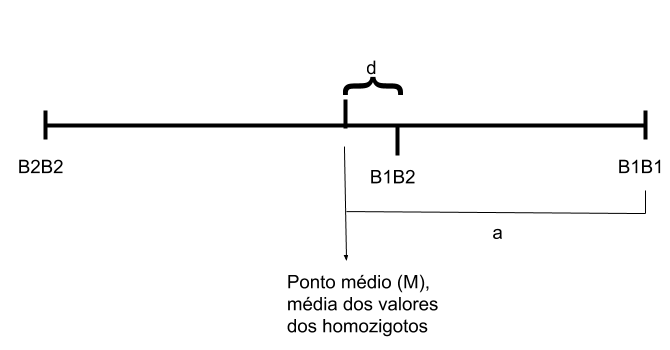
\includegraphics[width=0.9\linewidth]{img/grau-medio-dominancia.png}
  \caption{Grau Médio de Dominância}
  \label{fig:boat1}
\end{figure}


O valor do grau médio de dominância pode ser obtido dividindo-se d por a, esses valores são apresentados na \ref{fig:boat1}.


\begin{table}[H]
\centering
\begin{tabular}{l l }
\toprule
 \textbf{Resultado da Divisão} & \textbf{Interação Intra Alélica} \\
\midrule
 d/a = 0     & Interação  Aditiva  \\
 d/a = 1     & Dominância Completa \\
 0 < d/a < 1 & Dominância Parcial  \\
 d/a > 1     & Sobredominância     \\
\bottomrule
\end{tabular}
\caption{Genótipos Possíveis} \label{tab:t04}
\end{table}

O efeito de dominância mascara o processo de seleção, pois, ele dificulta o conhecimento dos indivíduos superiores pelos efeitos aditivos.

\section{Caráter Quantitativo}

O modelo para o estudo do caráter quantitativo é:

\begin{equation}
F = G + A
\end{equation}

Considere V(X) como a variância de X e Cov(X) como a covariância de X.

\begin{equation}
V(F) = V(G+A) \rightarrow V(F) = V(G) + V(A) + 2\times Cov(G+A)
\end{equation}

Como:

\begin{equation}
Cov(G+A) = 0
\end{equation}

Temos: 

\begin{equation}
V(F) = F(G+A) \rightarrow V(F) = V(G) + V(A) 
\end{equation}

A variância (V) é descrita pela seguinte fórmula: 

\begin{equation}
V(F) = \cfrac{\sum_{1}^{n} (x_i - \overline{X})^2}{n-1}
\end{equation}

ou

\begin{equation}
V(F) = \cfrac{\sum_{1}^{n} x^2 - [\sum_{1}^{n} x]^2}{n-1}
\end{equation}

\subsection{Dedução}

Para o cálculo da dedução da variância ambiental, considere um gene A, com dois alelos 'A' e 'a'.


\begin{table}[H]
\centering
\begin{tabular}{l l l l l}
\toprule
 \textbf{Genótipos} & \textbf{Nº Indivíduos} & \textbf{Frequência} & \textbf{Valor Genotípico} & \textbf{Val. Gen. Codificado} \\
\midrule
 AA & n1 & n1/n = D & X1 = u + a & a  \\
 Aa & n2 & n2/n = H & X2 = u + d & d  \\
 aa & n3 & n3/n = R & X3 = u - a & -a \\
\bottomrule
\end{tabular}
\caption{Dedução} \label{tab:t05}
\end{table}

Aplicando a fórmula da média na média genotípica:


\begin{definition}[Média Genotípica]
\begin{align}
&  Mg = \cfrac{\sum_{1}^{n} f_i\times{x_i}}{f_i} \\
&  Mg = D\times a + H\times d + R \times -a \\
&  Mg  = a \times (D-R) + H\times d \\
&  Mg = u + a\times(D-R) + H\times d
\end{align}
\end{definition}


\subsection{Variância Genética}

\begin{equation}
Va(x) = (\sum_{1}^{n} x_i^2) - (\sum_{1}^{n} f_i\times x_i)^2
\end{equation}

\begin{equation}
V(G) = D \times a^2 + H \times d^2 + R \times (-a)^2 - [a \times (D - R) + H \times d]^2
\end{equation}

\subsection{Estudo do Caráter}

Para o estudo do caráter, considere:

\begin{enumerate}
\item P1: AA
\item P2: aa
\item F1: Aa (P1xP2)
\item F2: [AA,Aa,aa]
\end{enumerate}


 
\begin{definition}[Análise de P1]

\begin{align}
&  Mg(P1) = u + a \times (D-R) + H \times d\\
&  Mg(P1) = u + a \times (1-0) + 0 \times d\\
&  Mg(P1) = u + a \\
\end{align}
\end{definition}

\begin{definition}[Variância de P1]

\begin{align}
&  V(P1) = D\times a^2 + H \times d^2 + R \times (-a)^2 - [ a \times (D-R) + H \times d ]^2 \\
&  V(P1) = 1\times a^2 + 0 \times d^2 + 0 \times (-a)^2 - [ a \times (1-0) + 0 \times d ]^2 \\
&  V(P1) = 1\times a^2 + -  1\times a^2 \\
&  V(P1) = 0
\end{align}

Portanto, como só existe um genótipo possível, não existe variância. A análise de P2 utiliza o mesmo método de P1, portanto, não há variância em P2.
\end{definition}


\begin{definition}[Análise de F2]

\begin{align}
&  Mg(F2) = u + a \times (\frac{1}{4}- \frac{1}{4}) + \frac{1}{2} \times d\\
&  Mg(F2) = u + \frac{1}{2} \times d\\
\end{align}
\end{definition}


\begin{definition}[Variância de F2]

\begin{align}
&  V(F2) = D\times a^2 + H \times d^2 + R \times (-a)^2 - [ a \times (D-R) + H \times d ]^2 \\
&  V(F2) = \frac{1}{4}\times a^2 + \frac{1}{2}\times d^2 + \frac{1}{4} \times (-a)^2 - [ a \times (\frac{1}{4}- \frac{1}{4}) + \frac{1}{2} \times d ]^2 \\
&  V(F2) = \frac{1}{4}\times a^2 + \frac{1}{2}\times d^2 + \frac{1}{4} \times (a)^2 - [ \frac{1}{2} \times d ]^2 \\
&  V(F2) = \frac{1}{2}\times a^2 + \frac{1}{2}\times d^2 - \frac{1}{4} \times d^2 \\
&  V(F2) = \frac{1}{2}\times a^2 + \frac{1}{4} \times d^2 \\
\end{align}
\end{definition}


\subsection{Variância Ambiental}

\begin{definition}[Fórmulas mais utilizadas]

\begin{align}
&  V(Amb) = V(P1) \\
&  V(Amb) = V(P2) \\
&  V(Amb) = V(F1) \\
&  V(Amb) = \frac{V(P1) + V(P2)}{2} \\
&  V(Amb) = \frac{V(P1) + V(P2) + V(F1)}{2} \\
&  V(Amb) = \frac{V(P1) + V(P2) + 2 \times V(F1)}{4} \\
\end{align}
\end{definition}



%----------------------------------------------------------------------------------------
%	CHAPTER 2
%----------------------------------------------------------------------------------------

\chapter{Parâmetros Genéticos}

\section{Herdabilidade}

A herdabilidade é um coeficiente que expressa a relação entre a variância genotípica e a variância fenotípica, ou seja, mede o nível da correspondência entre o fenótipo e o valor genético. 

\begin{definition}[Dedução de Herdabilidade]

\begin{align}
&  r = \frac{Cov(x,y)}{\sqrt{v(x) \times v(y)}} \\
&  r(F,G) = \frac{Cov(F,G)}{\sqrt{v(F) \times v(G)}} \\
&  r(F,G) = \frac{Cov(G+A,G)}{\sqrt{v(F) \times v(G)}} \\
&  r(F,G) = \frac{Cov(G,G) + Cov(G,A)}{\sqrt{v(F) \times v(G)}} \\
&  Como: Cov(G,A) = 0 \\
&  \rightarrow r(F,G) = \frac{Cov(G,G)}{\sqrt{v(F) \times v(G)}} \\
&  Como: Cov(X,X) = V(X) \\
&  \rightarrow r(F,G) = \frac{V(G)}{\sqrt{v(F) \times v(G)}} \\
&  r(F,G) = \sqrt{\frac{[V(G)]^2}{v(F) \times v(G)}} \\
&  r(F,G) = \sqrt{\frac{[V(G)]}{v(F)}} \\
&  Como: H = \frac{[V(G)]}{v(F)} \\
&  \rightarrow  r(F,G) = \sqrt{H^2} \\
\end{align}
\end{definition}


\begin{definition}[Fórmula da Herdabilidade]

\begin{align}
&  H^2 = \frac{V(G)}{V(F)} \\
\end{align}
\end{definition}

O valor da herdabilidade pode variar entre 0 e 1. Por definição, quando o valor da herdabilidade é maior que 0,7 é considerado alto para plantas. Em caso de animas, pode variar entre 0,3 e 0,4.



\subsection{Ganho de Seleção}

\begin{definition}[Fórmula do Ganho de Seleção (GS)]

\begin{align}
& GS = H^2 \times (\overline{X}_s - \overline{X}_0) \\
\end{align}
Sendo Xs a média dos indivíduos selecionados e X0 a média inicial dos indivíduos.
\end{definition}


\subsection{Média Predita}

\begin{definition}[Fórmula Média Predita (Xm)]

\begin{align}
& Xm = GS + \overline{X}_0 \\
\end{align}
\end{definition}


\subsection{Número de Genes}


\begin{definition}[Fórmula Número de Genes (Nrg)]

\begin{align}
& Nrg = \frac{(\overline{P_1} - \overline{P_2})^2}{8 \times V(G)_{F1}} \\
\end{align}
Sendo P1 a média dos parentais 1 e  P2 a média dos parentais 2 
\end{definition}



%
%----------------------------------------------------------------------------------------
%	CHAPTER 2
%----------------------------------------------------------------------------------------

\chapter{In-text Elements}

\section{Theorems}\index{Theorems}

This is an example of theorems.

\subsection{Several equations}\index{Theorems!Several Equations}
This is a theorem consisting of several equations.

\begin{theorem}[Name of the theorem]
In $E=\mathbb{R}^n$ all norms are equivalent. It has the properties:
\begin{align}
& \big| ||\mathbf{x}|| - ||\mathbf{y}|| \big|\leq || \mathbf{x}- \mathbf{y}||\\
&  ||\sum_{i=1}^n\mathbf{x}_i||\leq \sum_{i=1}^n||\mathbf{x}_i||\quad\text{where $n$ is a finite integer}
\end{align}
\end{theorem}

\subsection{Single Line}\index{Theorems!Single Line}
This is a theorem consisting of just one line.

\begin{theorem}
A set $\mathcal{D}(G)$ in dense in $L^2(G)$, $|\cdot|_0$. 
\end{theorem}

%------------------------------------------------

\section{Definitions}\index{Definitions}

This is an example of a definition. A definition could be mathematical or it could define a concept.

\begin{definition}[Definition name]
Given a vector space $E$, a norm on $E$ is an application, denoted $||\cdot||$, $E$ in $\mathbb{R}^+=[0,+\infty[$ such that:
\begin{align}
& ||\mathbf{x}||=0\ \Rightarrow\ \mathbf{x}=\mathbf{0}\\
& ||\lambda \mathbf{x}||=|\lambda|\cdot ||\mathbf{x}||\\
& ||\mathbf{x}+\mathbf{y}||\leq ||\mathbf{x}||+||\mathbf{y}||
\end{align}
\end{definition}

%------------------------------------------------

\section{Notations}\index{Notations}

\begin{notation}
Given an open subset $G$ of $\mathbb{R}^n$, the set of functions $\varphi$ are:
\begin{enumerate}
\item Bounded support $G$;
\item Infinitely differentiable;
\end{enumerate}
a vector space is denoted by $\mathcal{D}(G)$. 
\end{notation}

%------------------------------------------------

\section{Remarks}\index{Remarks}

This is an example of a remark.

\begin{remark}
The concepts presented here are now in conventional employment in mathematics. Vector spaces are taken over the field $\mathbb{K}=\mathbb{R}$, however, established properties are easily extended to $\mathbb{K}=\mathbb{C}$.
\end{remark}

%------------------------------------------------

\section{Corollaries}\index{Corollaries}

This is an example of a corollary.

\begin{corollary}[Corollary name]
The concepts presented here are now in conventional employment in mathematics. Vector spaces are taken over the field $\mathbb{K}=\mathbb{R}$, however, established properties are easily extended to $\mathbb{K}=\mathbb{C}$.
\end{corollary}

%------------------------------------------------

\section{Propositions}\index{Propositions}

This is an example of propositions.

\subsection{Several equations}\index{Propositions!Several Equations}

\begin{proposition}[Proposition name]
It has the properties:
\begin{align}
& \big| ||\mathbf{x}|| - ||\mathbf{y}|| \big|\leq || \mathbf{x}- \mathbf{y}||\\
&  ||\sum_{i=1}^n\mathbf{x}_i||\leq \sum_{i=1}^n||\mathbf{x}_i||\quad\text{where $n$ is a finite integer}
\end{align}
\end{proposition}

\subsection{Single Line}\index{Propositions!Single Line}

\begin{proposition} 
Let $f,g\in L^2(G)$; if $\forall \varphi\in\mathcal{D}(G)$, $(f,\varphi)_0=(g,\varphi)_0$ then $f = g$. 
\end{proposition}

%------------------------------------------------

\section{Examples}\index{Examples}

This is an example of examples.

\subsection{Equation and Text}\index{Examples!Equation and Text}

\begin{example}
Let $G=\{x\in\mathbb{R}^2:|x|<3\}$ and denoted by: $x^0=(1,1)$; consider the function:
\begin{equation}
f(x)=\left\{\begin{aligned} & \mathrm{e}^{|x|} & & \text{si $|x-x^0|\leq 1/2$}\\
& 0 & & \text{si $|x-x^0|> 1/2$}\end{aligned}\right.
\end{equation}
The function $f$ has bounded support, we can take $A=\{x\in\mathbb{R}^2:|x-x^0|\leq 1/2+\epsilon\}$ for all $\epsilon\in\intoo{0}{5/2-\sqrt{2}}$.
\end{example}

\subsection{Paragraph of Text}\index{Examples!Paragraph of Text}

\begin{example}[Example name]
\lipsum[2]
\end{example}

%------------------------------------------------

\section{Exercises}\index{Exercises}

This is an example of an exercise.

\begin{exercise}
This is a good place to ask a question to test learning progress or further cement ideas into students' minds.
\end{exercise}

%------------------------------------------------

\section{Problems}\index{Problems}

\begin{problem}
What is the average airspeed velocity of an unladen swallow?
\end{problem}

%------------------------------------------------

\section{Vocabulary}\index{Vocabulary}

Define a word to improve a students' vocabulary.

\begin{vocabulary}[Word]
Definition of word.
\end{vocabulary}

%----------------------------------------------------------------------------------------
%	PART
%----------------------------------------------------------------------------------------

\part{Part Two}

%----------------------------------------------------------------------------------------
%	CHAPTER 3
%----------------------------------------------------------------------------------------

\chapterimage{template/chapter_head_1.pdf} % Chapter heading image

\chapter{Presenting Information}

\section{Table}\index{Table}

\begin{table}[h]
\centering
\begin{tabular}{l l l}
\toprule
\textbf{Treatments} & \textbf{Response 1} & \textbf{Response 2}\\
\midrule
Treatment 1 & 0.0003262 & 0.562 \\
Treatment 2 & 0.0015681 & 0.910 \\
Treatment 3 & 0.0009271 & 0.296 \\
\bottomrule
\end{tabular}
\caption{Table caption}
\end{table}

%------------------------------------------------

\section{Figure}\index{Figure}

\begin{figure}[h]
\centering
\includegraphics[scale=0.5]{template/placeholder}
\caption{Figure caption}
\end{figure}


%----------------------------------------------------------------------------------------
%	BIBLIOGRAPHY
%----------------------------------------------------------------------------------------

\chapter*{Bibliografia}
%\addcontentsline{toc}{chapter}{\textcolor{ocre}{Bibliography}}
%\section*{Books}
%\addcontentsline{toc}{section}{Books}
%\printbibliography[heading=bibempty,type=book]
%\section*{Articles}
%\addcontentsline{toc}{section}{Articles}
%\printbibliography[heading=bibempty,type=article]

%----------------------------------------------------------------------------------------
%	INDEX
%----------------------------------------------------------------------------------------

\cleardoublepage
\phantomsection
\setlength{\columnsep}{0.75cm}
\addcontentsline{toc}{chapter}{\textcolor{ocre}{Index}}
\printindex

%----------------------------------------------------------------------------------------

\end{document}